\setlength{\parindent}{0em}

The procedures to determine the ambient temperature axial compression capacity of stud based on Direct Strength Method is shown below.

\subsection*{Nominal External Dimensions}

\begin{figure}[!htbp]
    \centering
    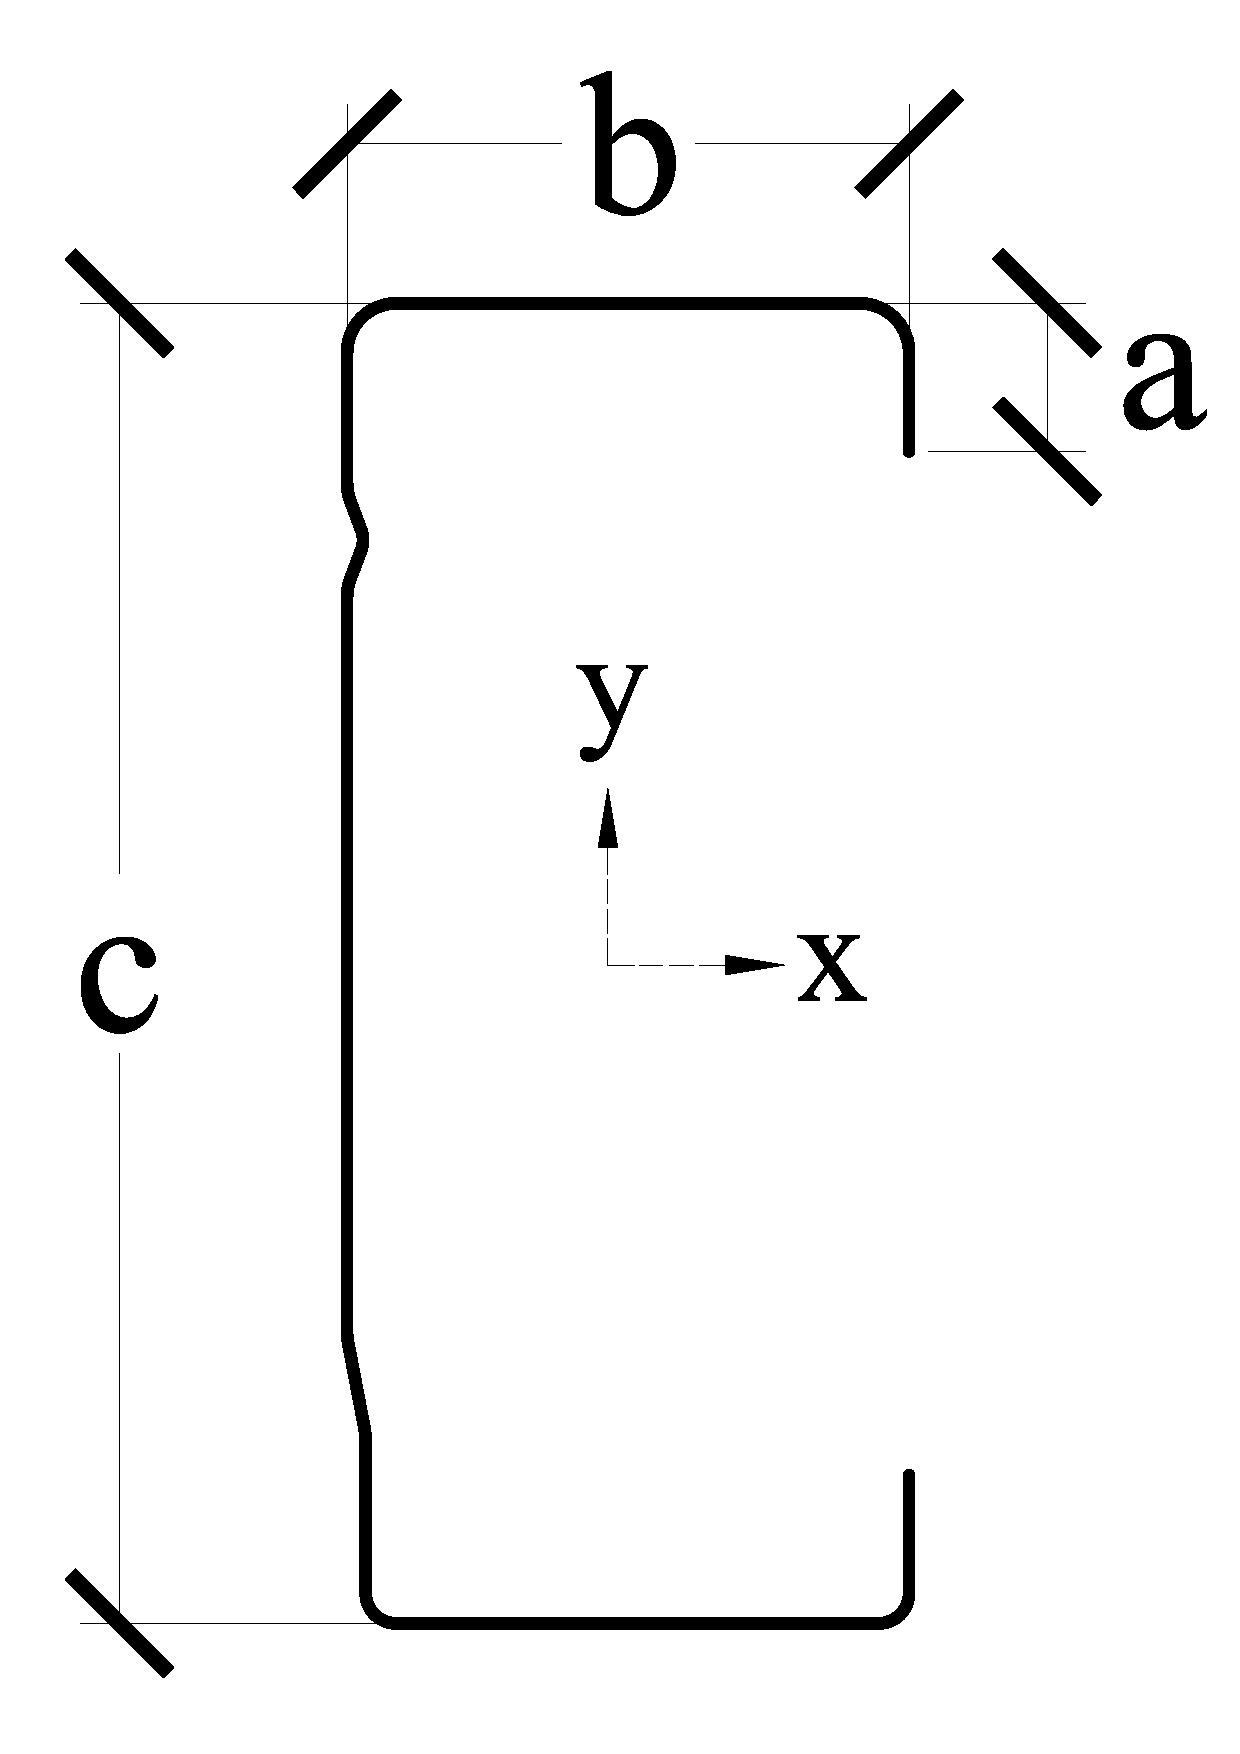
\includegraphics[scale=0.15]{dsm-drawing.pdf}
    \caption{Nominal external dimensions of stud}
    \label{fig:dsm-drawing}
\end{figure}

A = 7 mm, B = 36 mm and C = 89 mm; Thickness (BMT) = 0.95 mm

Effective length about the major axis of bending $L_x$ = 3,000 mm

Effective length about the minor axis of bending $L_x$ = 1,000 mm

\subsection*{Section Properties of Stud from CUFSM}

Gross area of section $A_g$ = 160.34 $mm^2$

Second moment of area about the major axis $I_{xx}$ = 202,187 $mm^4$

Second moment of area about the minor axis $I_{yy}$ = 26,513 $mm^4$

Radius of gyration about major axis $r_x$ = $\sqrt{\dfrac{I_{xx}}{A_g}}$ = $\sqrt{\dfrac{202,187}{160.34}}$ = 35.51 mm

Radius of gyration about minor axis $r_y$ = $\sqrt{\dfrac{I_{yy}}{A_g}}$ = $\sqrt{\dfrac{26,513}{160.34}}$ = 12.86 mm

\subsection*{Mechanical Properties of the Stud}

Yield strength at ambient temperature (measured) $f_y$ = 617.5 MPa 

Elastic modulus at ambient temperature (measured) $E_20$ = 215,500 MPa

\subsection*{Elastic flexural buckling stress ($f_{oc}$) - Cl 3.4 AS/NZS (\citet{ASNZ4600})}

PLasterboard provides torsional and flexural-torsional buckling restraints to the studs in gypsum plasterboard lined walls, thus the stud sections are not subjected to torsional or flexural-torsional buckling.

\subsubsection*{Elastic flexural buckling stress about the major axis $f_{ox}$}

\begin{equation*}
    f_{ox} = \dfrac{\pi^2E}{\left(\dfrac{l_{ex}}{r_x}\right)^2} = \dfrac{\pi^2 \times 215,500}{\left(\dfrac{3000}{35.51}\right)^2} = 297.99MPa
\end{equation*}

\subsubsection*{Elastic flexural buckling stress about the minor axis $f_{oy}$}

\begin{equation*}
    f_{ox} = \dfrac{\pi^2E}{\left(\dfrac{l_{ex}}{r_y}\right)^2} = \dfrac{\pi^2 \times 215,500}{\left(\dfrac{1000}{12.86}\right)^2} = 351.68 MPa
\end{equation*}

Elastic flexural buckling stress $f_{oc}$ = Lesser of $f_{ox}$ and $f_{oy}$ = 297.99 MPa

\subsubsection*{Flexural buckling capacity of the stud $N_{ce}$}

Elastic flexural buckling load $N_{oc}$ = $A_g$$f_{oc}$ = 160.34 $\times$ 297.99 = 47.78 kN

Nominal yield load $N_y$ = $A_g$$f_y$ = 160.34 $\times$ 617.5 = 99.01 kN

\begin{equation*}
    \lambda_c = \sqrt{\dfrac{N_y}{N_{oc}}} = \sqrt{\dfrac{99.01}{47.78}} = 1.440<1.5
\end{equation*}

Flexural buckling capacity $N_{ce}$ = $(0.658^{\lambda_C^2})N_y$ = $0.658^{{1.44}^{2}} \times 99.01$ = 41.59 kN

\subsection*{Local buckling capacity of the stud}

Local buckling factor = 0.22 (From CUFSM signature curve)

Critical local buckling load $N_{ol}$ = $A_g$ $\times$ (Locl buckling load factor) $\times$ $f_y$
\begin{equation*}
    N_{ol} = 160.34 \times (0.22 \times 617.5) = 21.85 kN
\end{equation*}
\begin{equation*}
    \lambda_l = \sqrt{\dfrac{N_{ce}}{N_{ol}}}
    = \sqrt{\dfrac{41.59}{21.85}} = 1.379 > 0.776
\end{equation*}

Local buckling capacity of the stud $N_{cl,1}$ = $\left(1-0.15\left(\dfrac{N_{ol}}{N_{ce}}\right)^{0.4}\right)\left(\dfrac{N_{ol}}{N_{ce}}\right)^{0.4}N_{ce}$
\begin{equation*}
    N_{cl,1} = \left(1-0.15\left(\dfrac{21.85}{41.59}\right)^{0.4}\right)\left(\dfrac{21.58}{41.59}\right)^{0.4} \times 41.59 = 28.43 kN
\end{equation*}

Ultimate local buckling capacity of the stud at ambient temperature = \textbf{28.43 kN}

% If flexural, torsional and flexural-torsional buckling modes are restrained, the local local buckling capacity of the stud is:

% \begin{equation*}
%     \lambda_l = \sqrt{\dfrac{N_y}{N_{ol}}}
%     = \sqrt{\dfrac{71.36}{9.28}} = 2.774 > 0.776
% \end{equation*}

% Local buckling capacity of the stud $N_{cl,2}$ = $\left(1-0.15\left(\dfrac{N_{ol}}{N_y}\right)^{0.4}\right)\left(\dfrac{N_{ol}}{N_y}\right)^{0.4}N_y$
% \begin{equation*}
%     N_{cl,2} = \left(1-0.15\left(\dfrac{9.28}{71.36}\right)^{0.4}\right)\left(\dfrac{9.28}{71.36}\right)^{0.4} \times 71.36 = 29.46 kN
% \end{equation*}

% Ultimate capacity of the stud at ambient temperature = \textbf{17.50 kN} (Local + flexural buckling modes)